\cohead{\Large\textbf{Allgemeine Sinus-/Cosinusfunktion}}
\fakesubsection{Allgemeine Sinus- und Cosinusfunktion}
Die allgemeine Sinusfunktion bzw. Cosinusfunktion sind gegeben durch:
\[f(x)=a\sin\left(bx\right)+d\qquad g(x)=a\cos\left(bx\right)+d\]
\begin{itemize}
	\item \(a\): \textcolor{loes}{Streckfaktor relativ zum Mittelwert in \(y\)-Richtung. Der Betrag von \(a\) gibt die Amplitude an.}\\
	\item \(d\): \textcolor{loes}{Verschiebung in \(y\)-Richtung. Da der Mittelwert zuvor bei \(0\) lag, entspricht \(d\) dem Mittelwert.}\\
	\item \(b\): \textcolor{loes}{Streckfaktor in \(x\)-Richtung. Zwischen dem Streckfaktor und der Periode \(p\) besteht folgender Zusammenhang: \(b\cdot p=2\pi\).}\\
\end{itemize}
Beispiel: \(\displaystyle f(x)=2\sin\left(0,5x\right)-1\)\\
\begin{minipage}{\textwidth}
	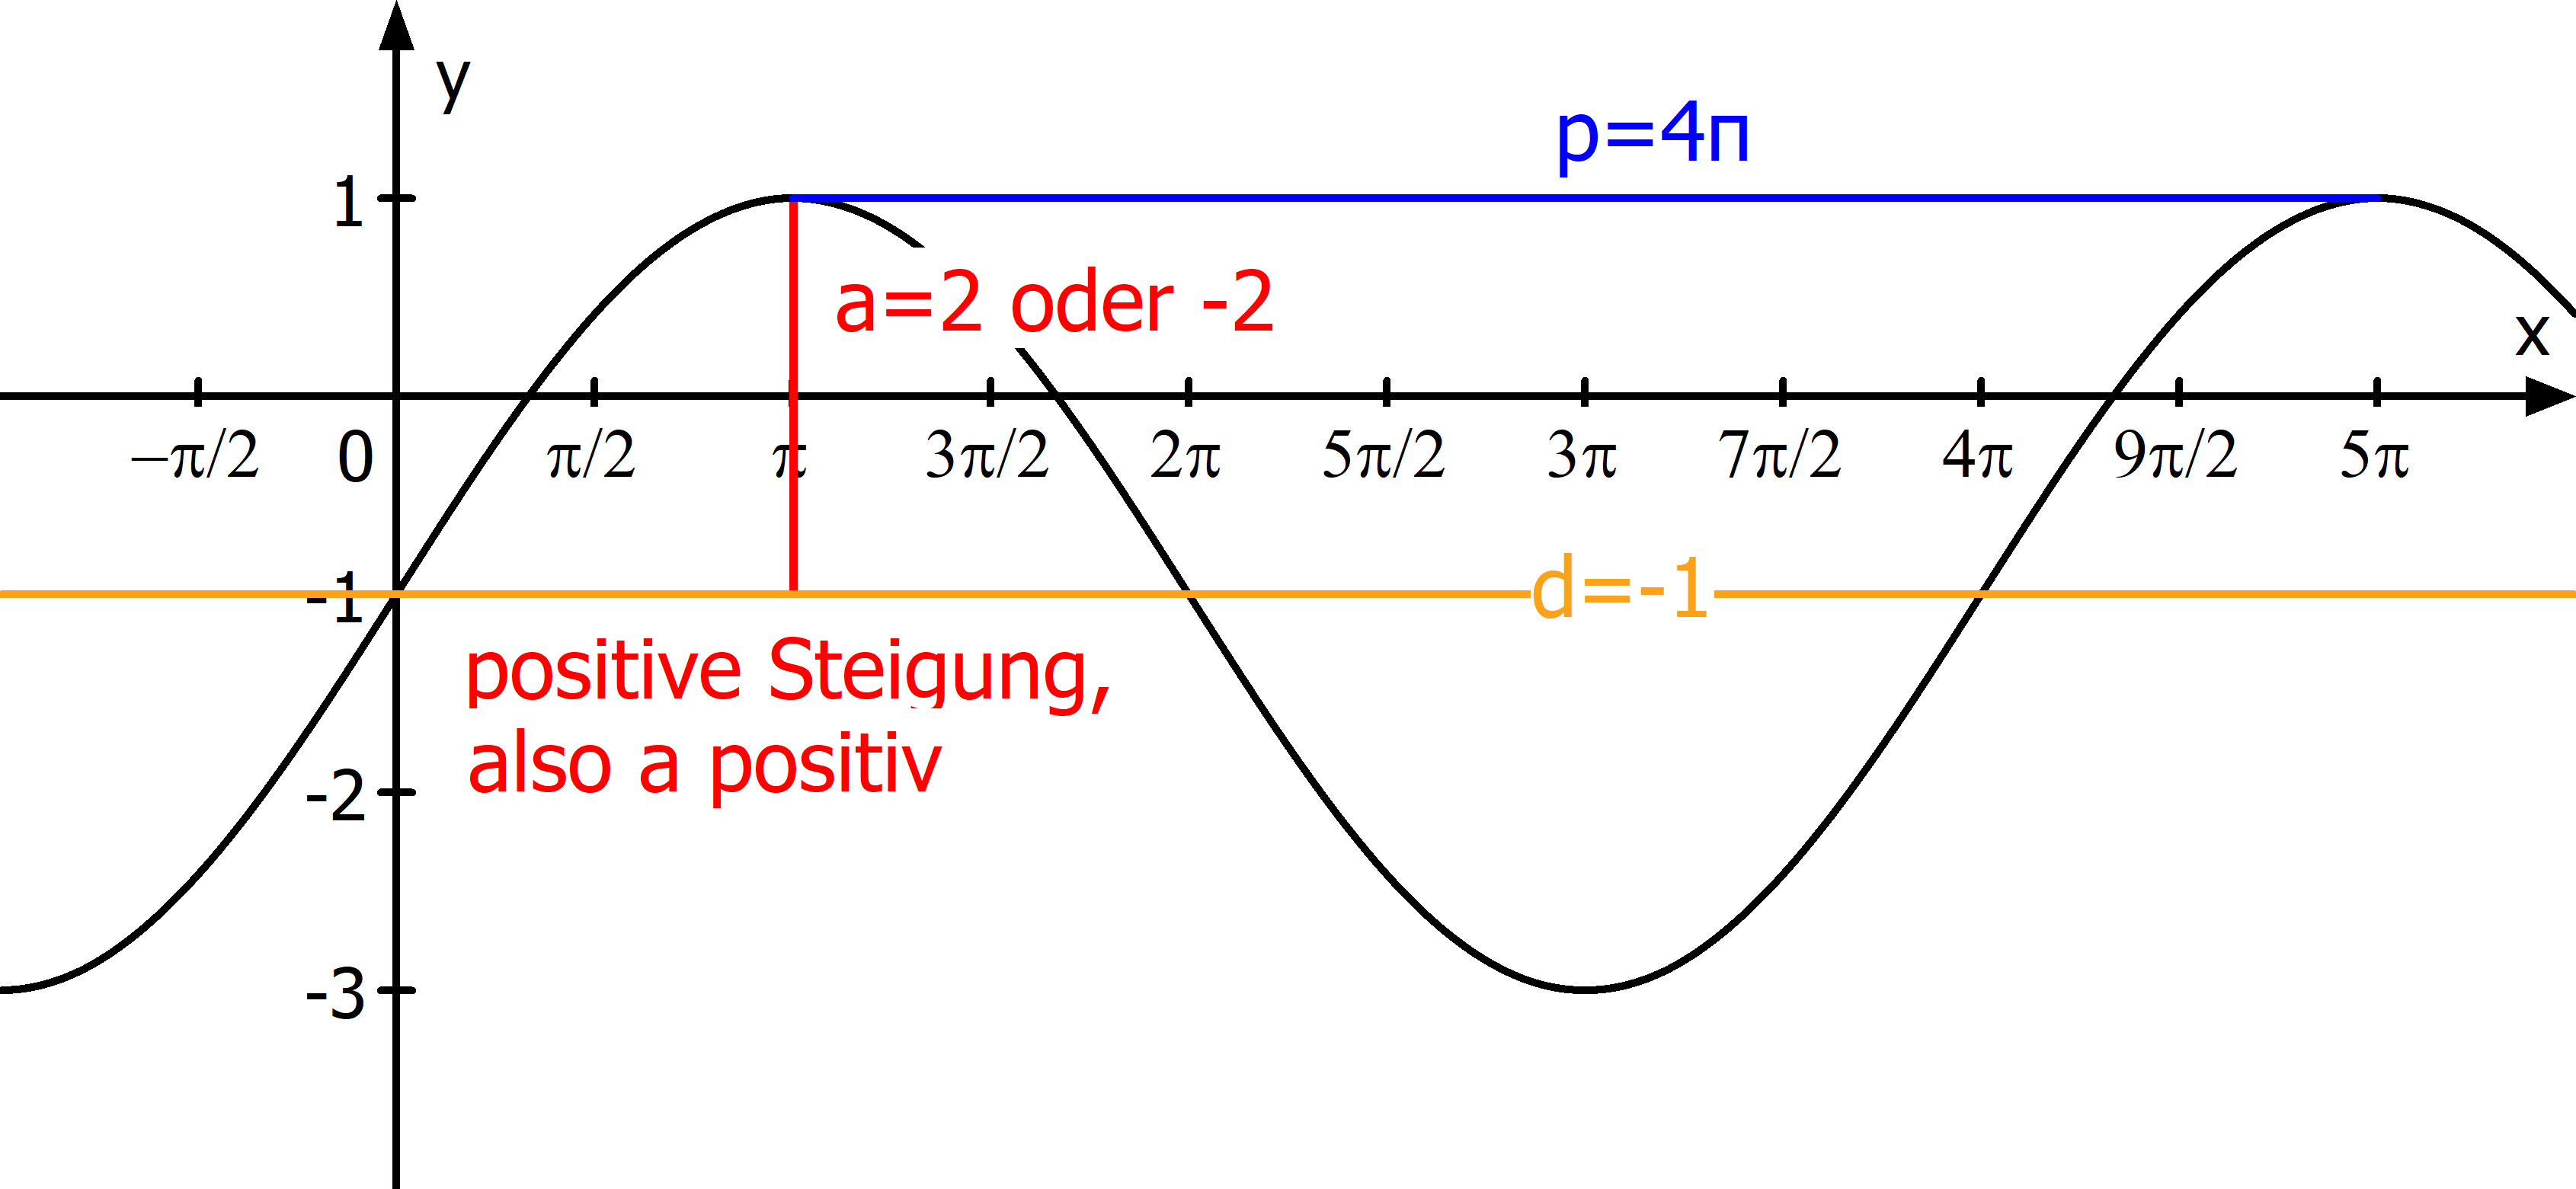
\includegraphics[width=.95\linewidth]{\trigonometrie/pics/AllgSin.png}\\
\end{minipage}\\
Beispiel: \(\displaystyle g(x)=-0,5\cos\left(\pi x\right)+1\)\\
\begin{minipage}{\textwidth}
	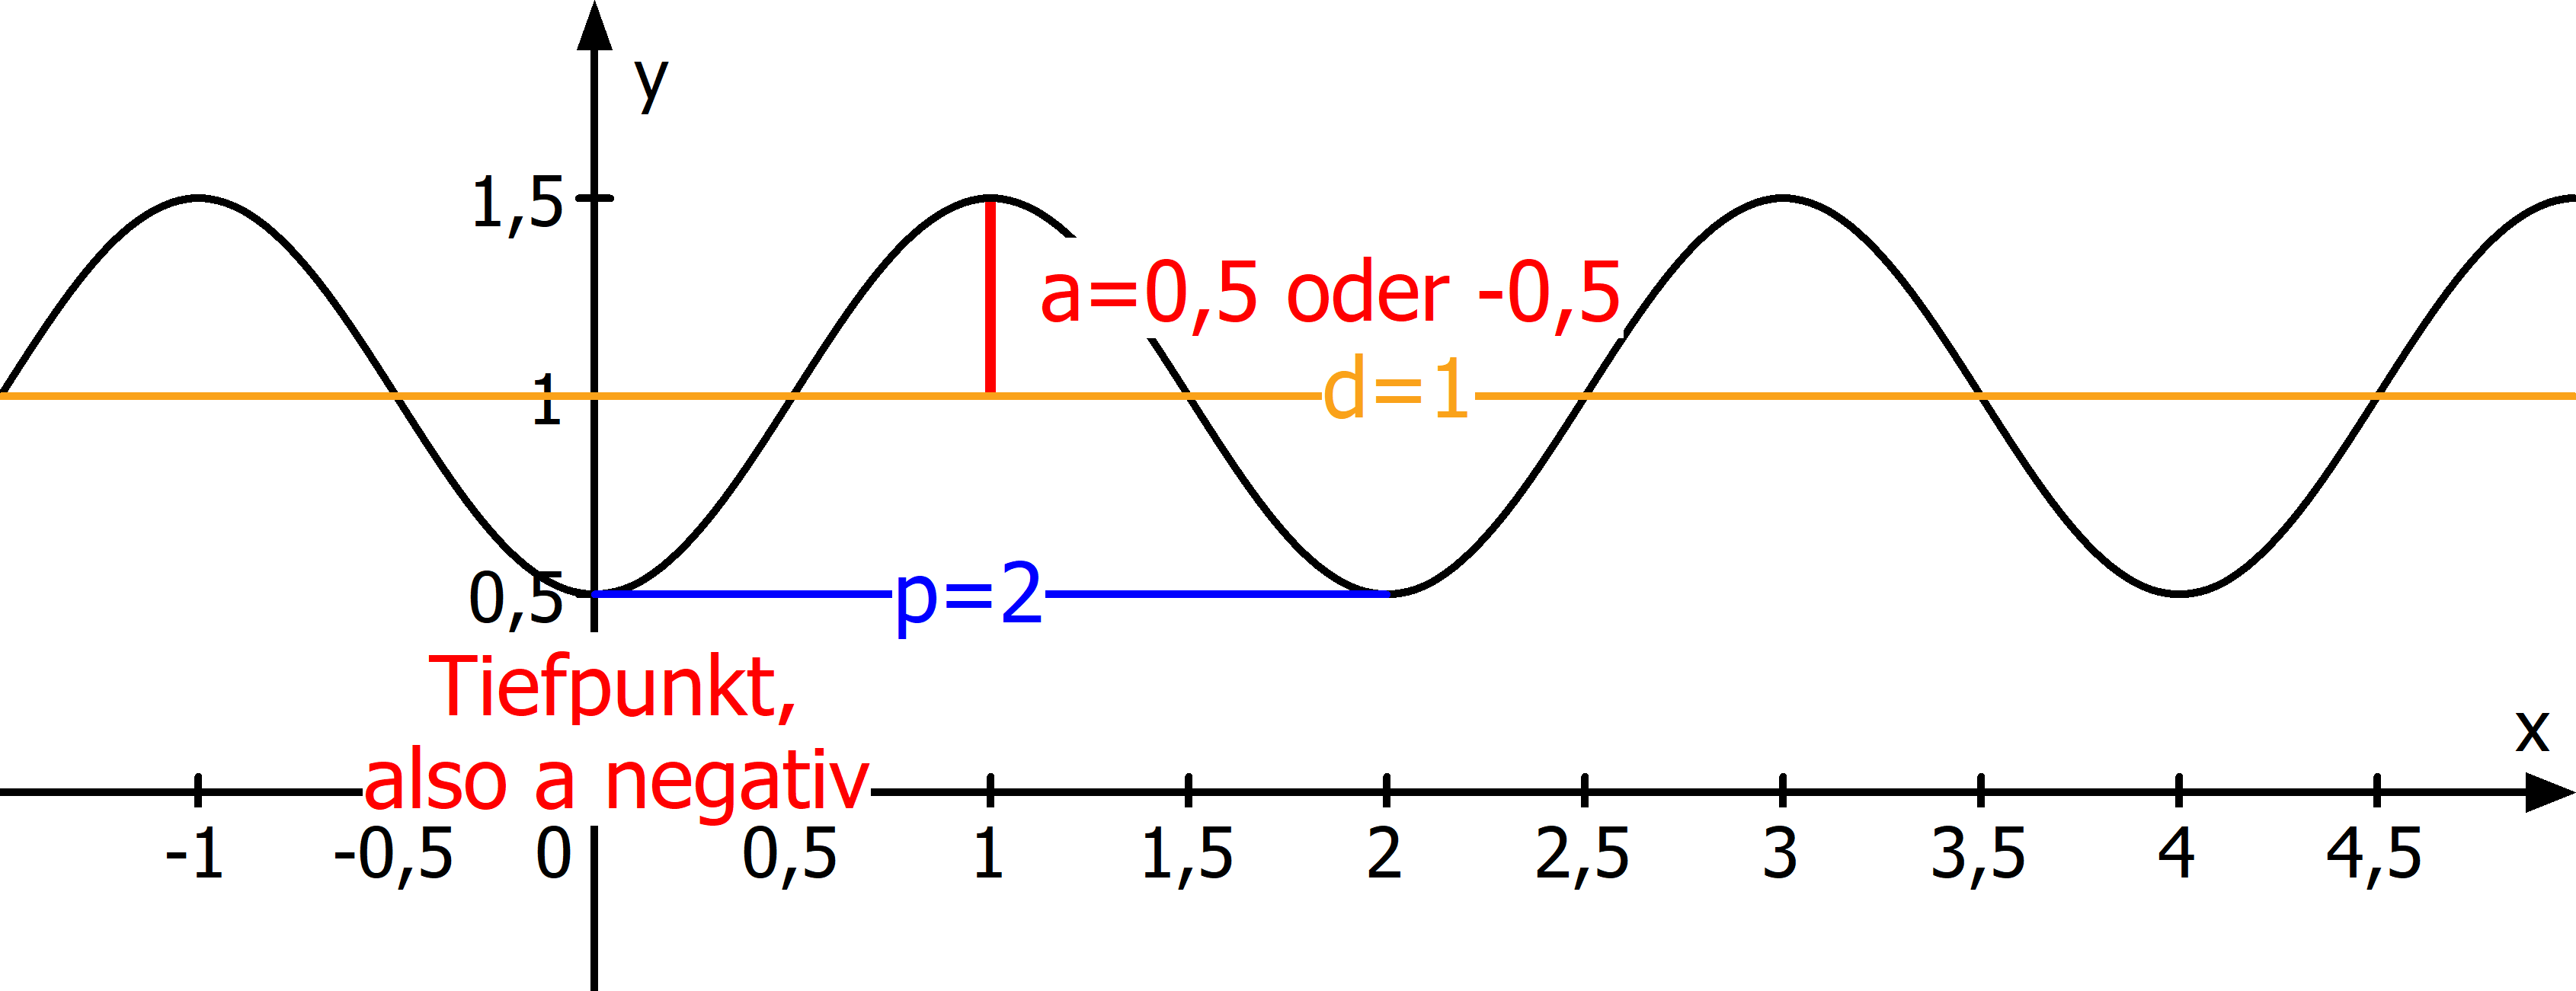
\includegraphics[width=.95\linewidth]{\trigonometrie/pics/AllgCos.png}\\
\end{minipage}\\
\newpage
\textbf{Bestimmen der Nullstellen:}\\
Die Nullstellen sind an sich nicht schwer zu bestimmen. Das Problem ist, dass es unendlich viele Nullstellen gibt. Will man alle Nullstellen aufschreiben, so braucht man eine neue Notation. Das gleiche Problem ergibt sich bei den Maxima, Minima und Wendestellen.
\begin{tcolorbox}
	\textbf{Notation für unendlich viele Stellen:}\\
	Erinnerung: Die ganzen Zahlen sind wie folgt definiert: \(\Z=\{0,\ 1,\ -1,\ 2,\ -2,\ 3,\ -3,\dots\}\)
	\textcolor{loestc}{Zur Notation nutzen wir aus, dass sich die Nullstellen/Maxima/Minima/Wendestellen in festen Abständen wiederholen, z.B. wieder beträgt der Abstand von einer Nullstelle zur nächsten bei sowohl \(\sin x\) als auch \(\cos x\)	jeweils \(\pi\):
		\[\text{alle Stellen }=\text{ eine Stelle }+\ k\cdot\text{Abstand der Stellen, }k\in\Z\]
		Bsp.: Nullstellen von \(\sin x\): \(x_k=0+k\cdot \pi,\ k\in\Z\)
	}
\end{tcolorbox}

\begin{Exercise}[title={\raggedright\normalfont Gib jeweils die Amplitude, die Periode und den Mittelwert an. Skizziere dann das Schaubild so, dass mindestens eine Periode zu sehen ist.}, label=allgSinCosA1]
	\begin{enumerate}[label=\alph*)]
		\item \(f_1(x)=-2\sin\left(3x\right)-4\)
		\item \(f_2(x)=1,5\sin\left(4x\right)-2\)
		\item \(f_3(x)=-3\cos\left(0,5x\right)+1\)
		\item \(f_4(x)=\cos\left(\frac{1}{3}x\right)\)
		\item \(f_5(x)=-\sin\left(\frac{1}{2}x\right)-1\)
		\item \(f_6(x)=3\sin\left(\frac{2}{3}x\right)+3\)
		\item \(f_7(x)=4\cos\left(\frac{3}{4}x\right)+2\)
		\item \(f_8(x)=2,5\sin\left(\pi x\right)-1\)
		\item \(f_9(x)=-\cos\left(\frac{\pi}{2}x\right)+2\)
		\item \(f_{10}(x)=-4\sin\left(2\pi x\right)-1\)
		\item \(f_{11}(x)=-2,5\cos\left(4\pi x\right)+3,5\)
		\item \(f_{12}(x)=3\cos\left(1,5x\right)+2\)
		\item \(f_{13}(x)=0,5\sin\left(0,5\pi x\right)+1,5\)
		\item \(f_{14}(x)=-5\sin\left(4\pi x\right)-3\)
		\item \(f_{15}(x)=3\cos\left(x\right)+2\)
		\item \(f_{16}(x)=-2\sin\left(2x\right)\)
		\item \(f_{17}(x)=2,5\sin\left(2x\right)-3,5\)
		\item \(f_{18}(x)=3,5\cos\left(\frac{2}{3}\pi x\right)+2\)
		\item \(f_{19}(x)=5\cos\left(x\right)-4\)
		\item \(f_{20}(x)=-6\cos\left(2\pi x\right)+10\)
	\end{enumerate}
\end{Exercise}
\newpage
%%%%%%%%%%%%%%%%%%%%%%%%%%%%%%%%%%%%%%%%%%%%%%%%%%%%%%%%%%%%%%%%%%%%%%%%%%%%%%%%%%%%%%%%%%%%%%%%%%%%%%%%%%%%%%%%%%%%%%%%
\begin{Exercise}[title={Stelle jeweils die Funktionsgleichung vom Typ \(a\cdot \sin\left(bx\right)+d\)\\oder \(a\cdot \cos\left(bx\right)+d\) auf.}, label=allgSinCosA2]\\
	\begin{minipage}{\textwidth}
		\begin{minipage}{0.49\textwidth}
			\begin{enumerate}[label=\alph*)]
				\item \begin{minipage}{.9\textwidth}
					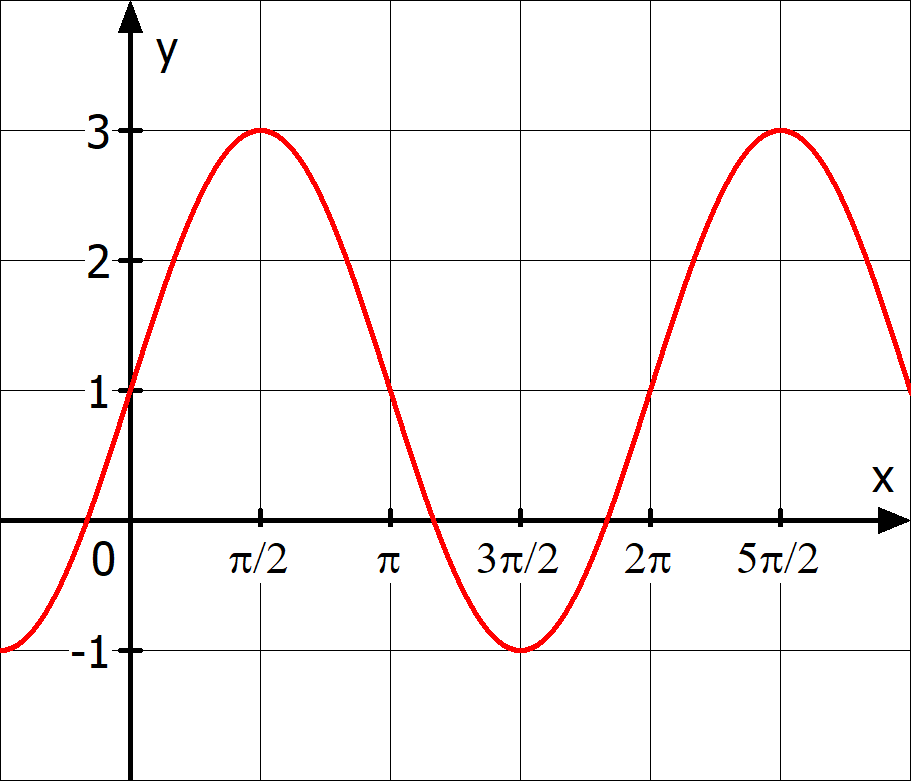
\includegraphics[width=.75\linewidth]{\trigonometrie/pics/AllgSinA2_1.png}\\
				\end{minipage}	
				\item \begin{minipage}{.9\textwidth}
					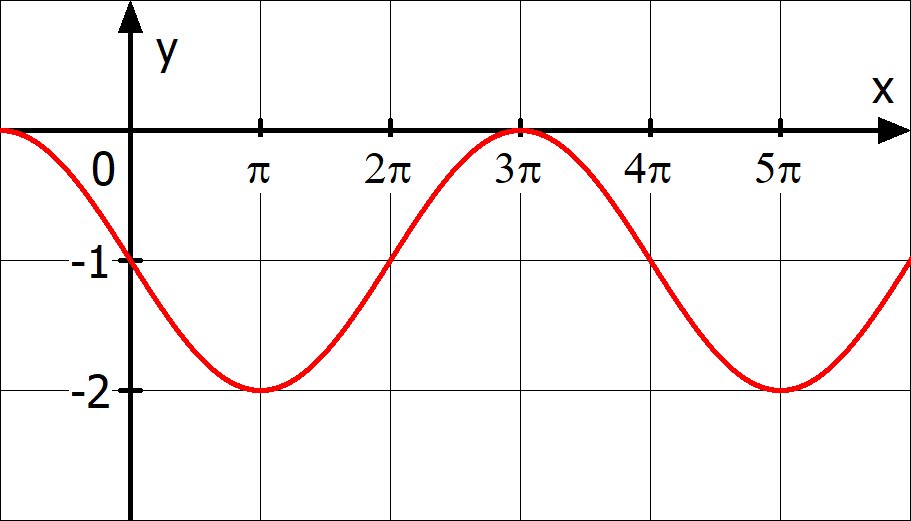
\includegraphics[width=.75\linewidth]{\trigonometrie/pics/AllgSinA2_2.png}\\
				\end{minipage}
				\item \begin{minipage}{.9\textwidth}
					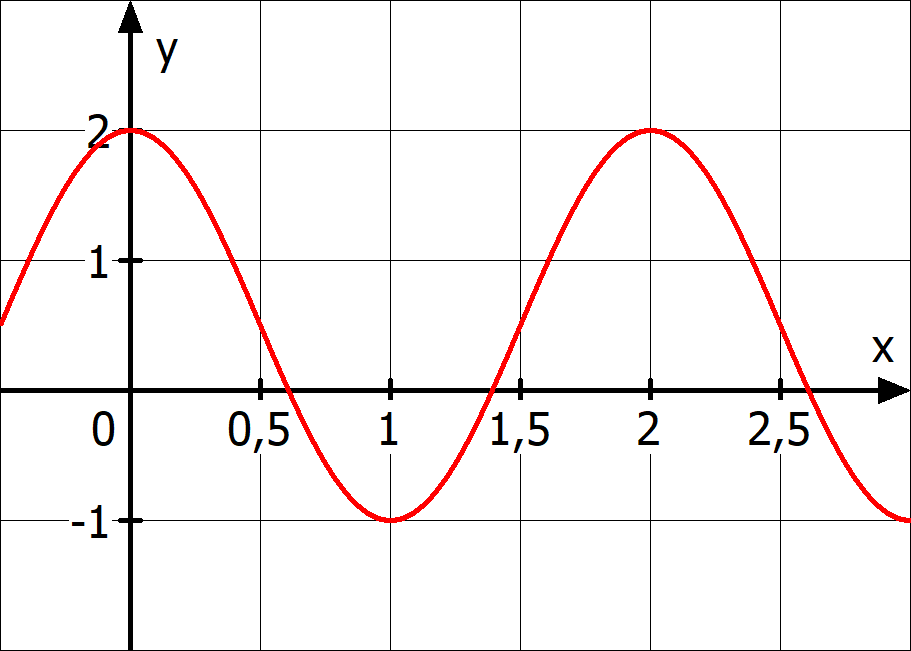
\includegraphics[width=.75\linewidth]{\trigonometrie/pics/AllgSinA2_3.png}\\
				\end{minipage}
				\item \begin{minipage}{.9\textwidth}
					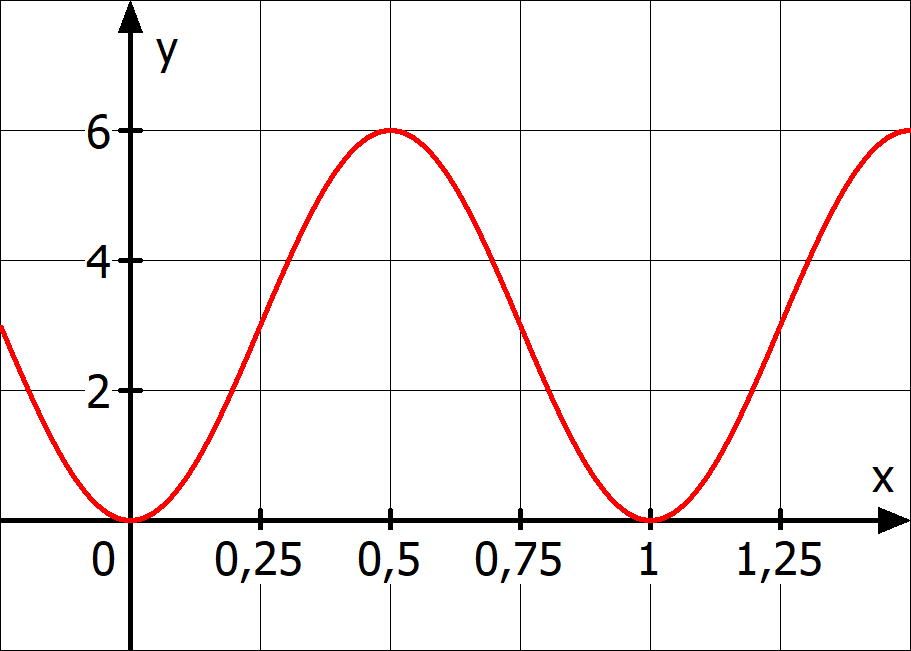
\includegraphics[width=.75\linewidth]{\trigonometrie/pics/AllgSinA2_4.png}\\
				\end{minipage}
				\item \begin{minipage}{.9\textwidth}
					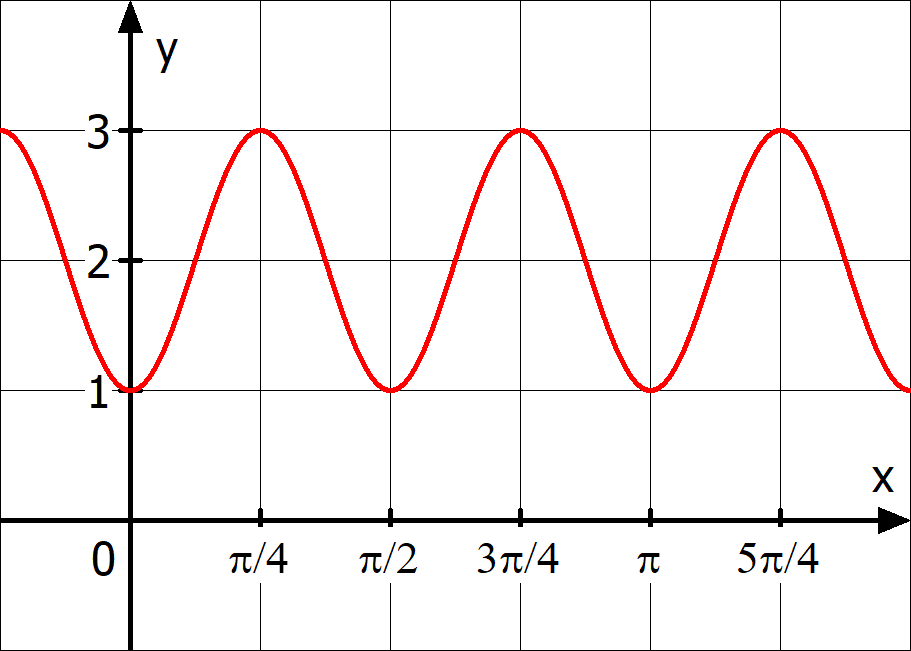
\includegraphics[width=.75\linewidth]{\trigonometrie/pics/AllgSinA2_5.png}\\
				\end{minipage}
			\end{enumerate}
		\end{minipage}
		\begin{minipage}{0.49\textwidth}
			\begin{enumerate}[label=\alph*)]
				\setcounter{enumi}{5}
				\item \begin{minipage}{.9\textwidth}
					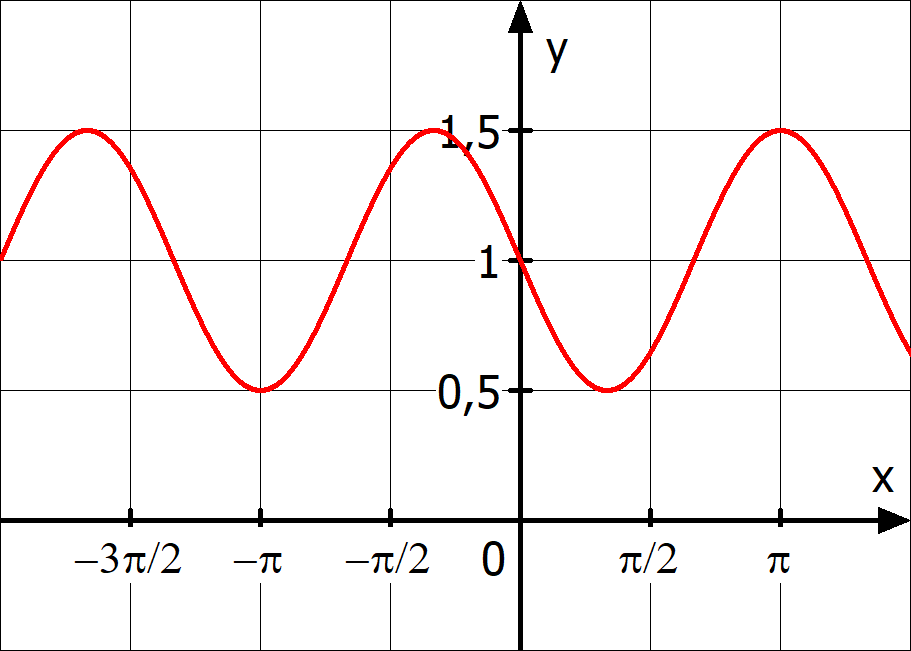
\includegraphics[width=.75\linewidth]{\trigonometrie/pics/AllgSinA2_6.png}\\
				\end{minipage}	
				\item \begin{minipage}{.9\textwidth}
					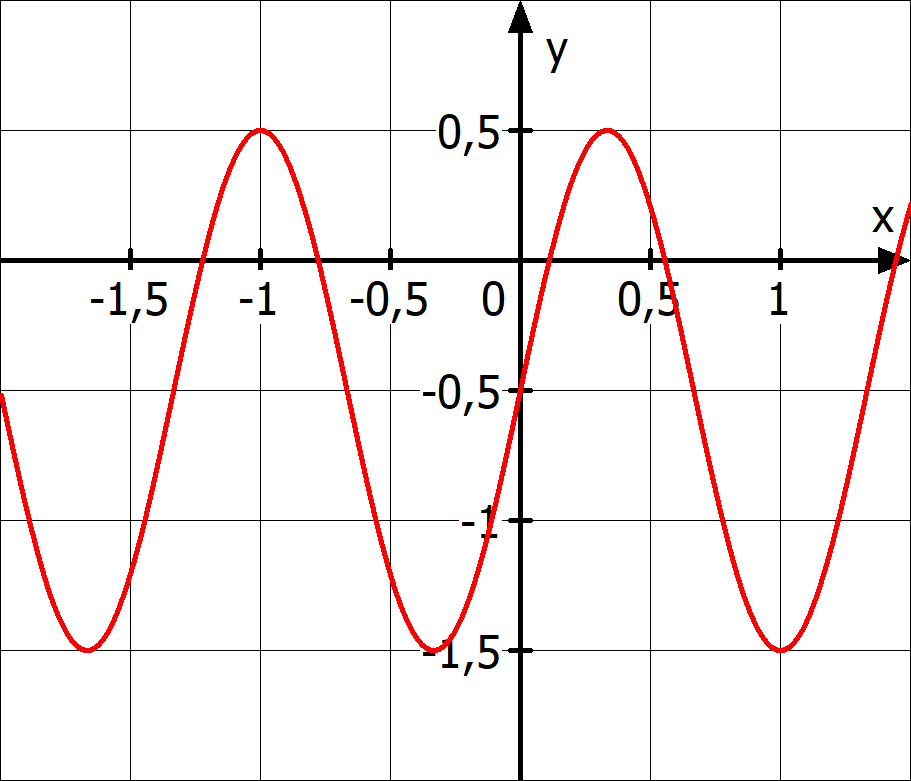
\includegraphics[width=.75\linewidth]{\trigonometrie/pics/AllgSinA2_7.png}\\
				\end{minipage}
				\item \begin{minipage}{.9\textwidth}
					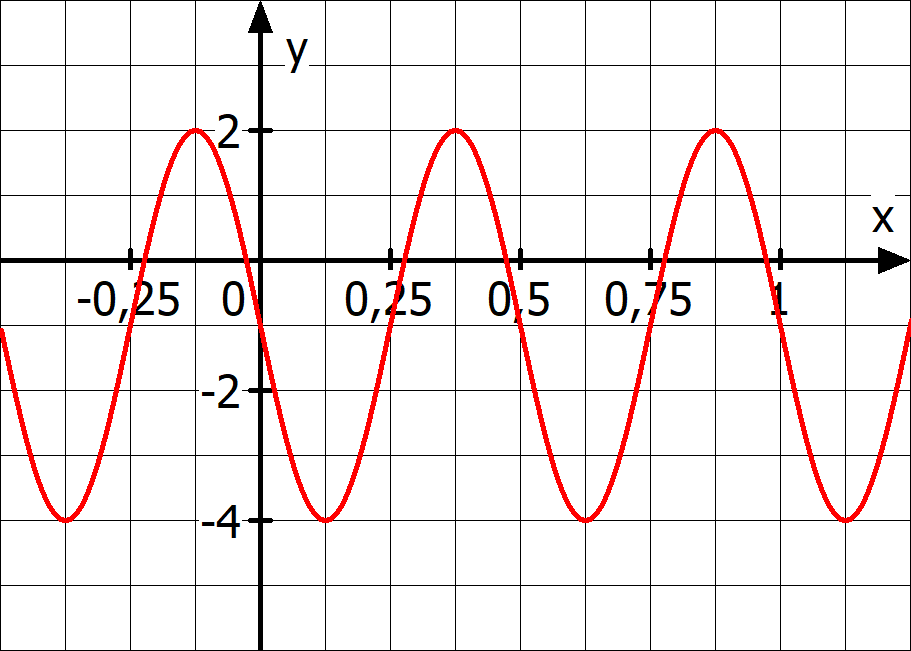
\includegraphics[width=.75\linewidth]{\trigonometrie/pics/AllgSinA2_8.png}\\
				\end{minipage}
				\item \begin{minipage}{.9\textwidth}
					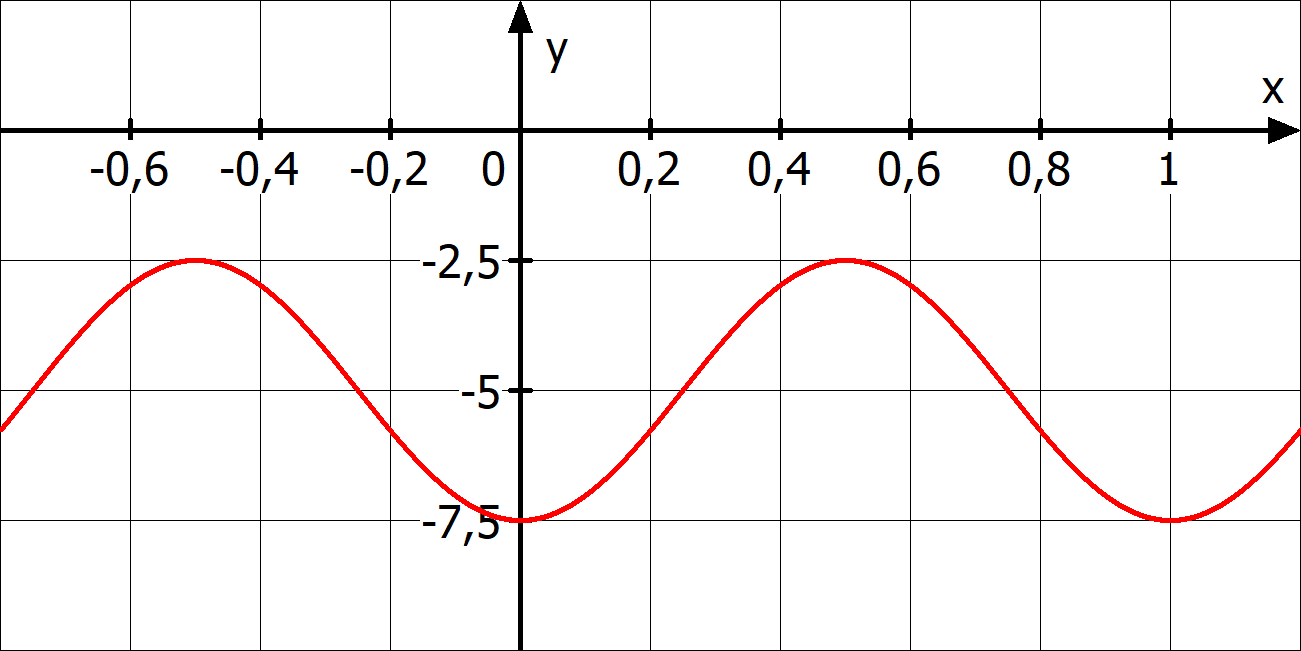
\includegraphics[width=.75\linewidth]{\trigonometrie/pics/AllgSinA2_9.png}\\
				\end{minipage}
				\item \begin{minipage}{.9\textwidth}
					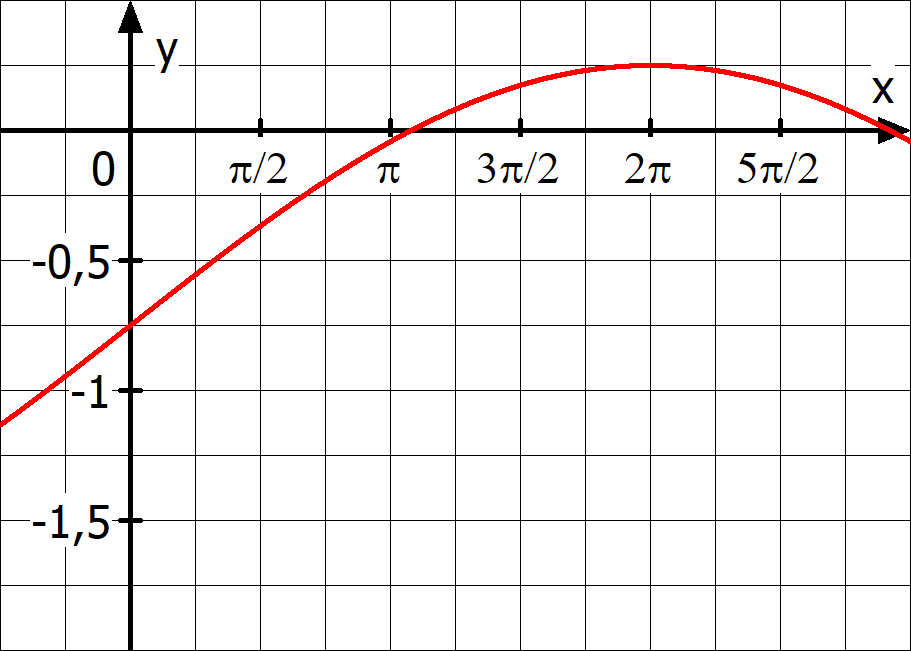
\includegraphics[width=.75\linewidth]{\trigonometrie/pics/AllgSinA2_10.png}\\
				\end{minipage}
			\end{enumerate}
		\end{minipage}
	\end{minipage}
\end{Exercise}


%%%%%%%%%%%%%%%%%%%%%%%%%%%%%%%%%%%%%%%%%
\begin{Answer}[ref=allgSinCosA1]
	\begin{enumerate}[label=\alph*)]
		\item Amplitude \(a_{1}=2\), Periode \(p_{1}=\frac{2\pi}{3}\), Mittelwert \(d_{1}=-4\)\\
		\begin{minipage}{\textwidth}
			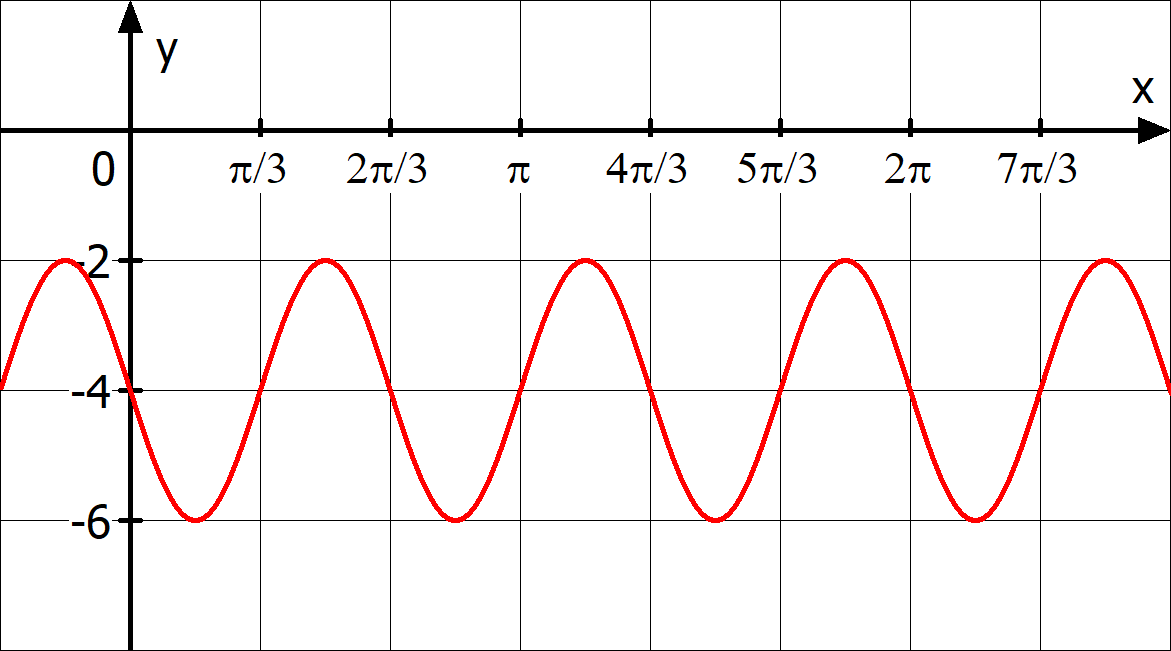
\includegraphics[height=5cm]{\trigonometrie/pics/AllgSinA1_1.png}\\
		\end{minipage}	 
		\item Amplitude \(a_{2}=1,5\), Periode \(p_{2}=\frac{\pi}{2}\), Mittelwert \(d_{2}=-2\)\\
		\begin{minipage}{\textwidth}
			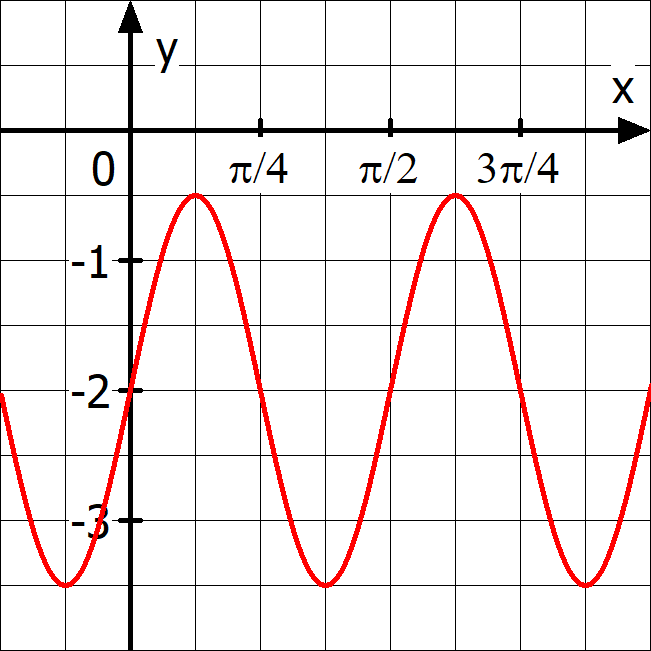
\includegraphics[height=5cm]{\trigonometrie/pics/AllgSinA1_2.png}\\
		\end{minipage}	 
		\item Amplitude \(a_{3}=3\), Periode \(p_{3}=4\pi\), Mittelwert \(d_{3}=1\)\\
		\begin{minipage}{\textwidth}
			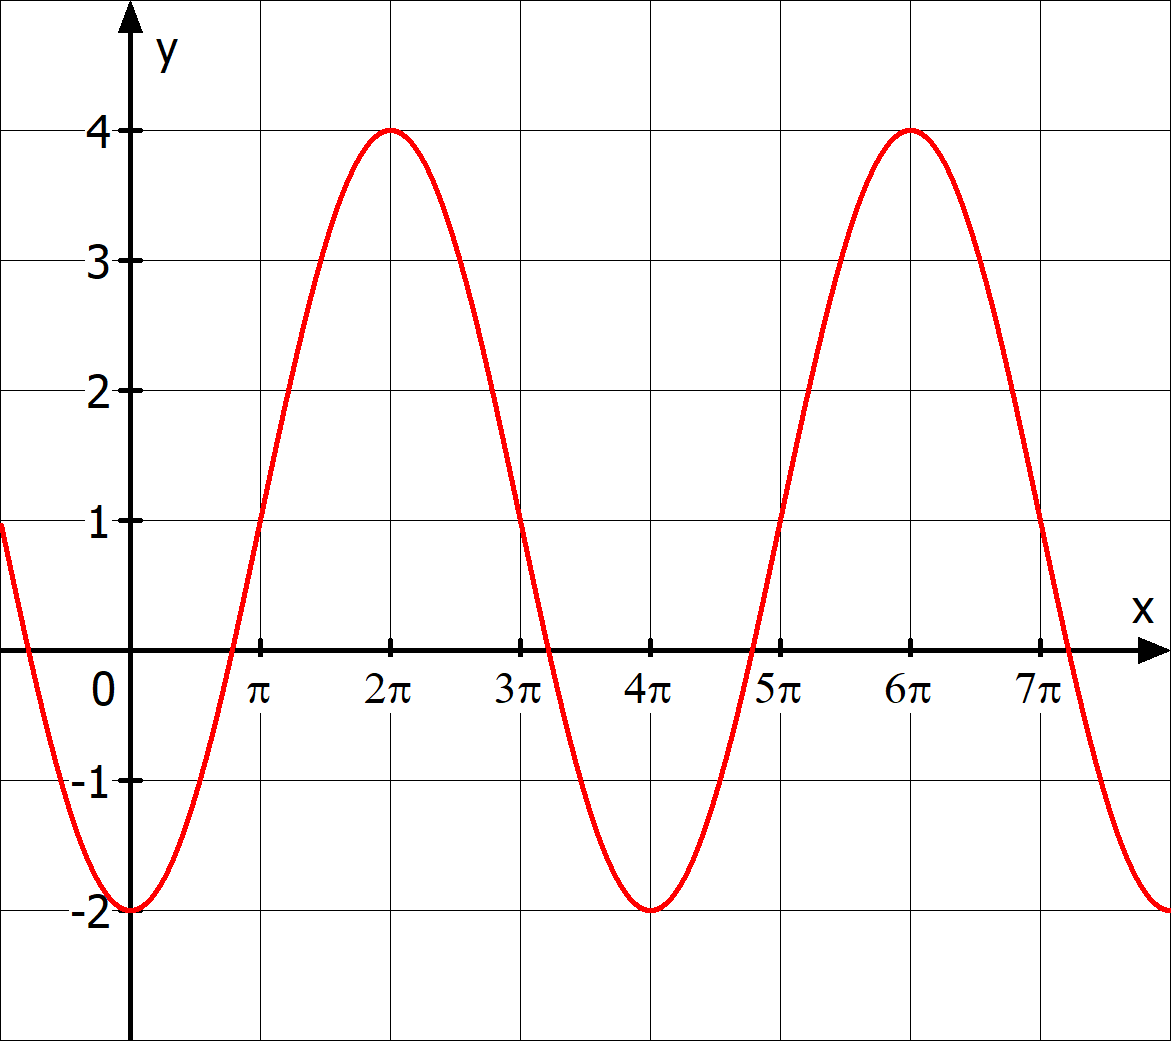
\includegraphics[height=5cm]{\trigonometrie/pics/AllgSinA1_3.png}\\
		\end{minipage}	 
		\item Amplitude \(a_{4}=1\), Periode \(p_{4}=6\pi\), Mittelwert \(d_{4}=0\)\\
		\begin{minipage}{\textwidth}
			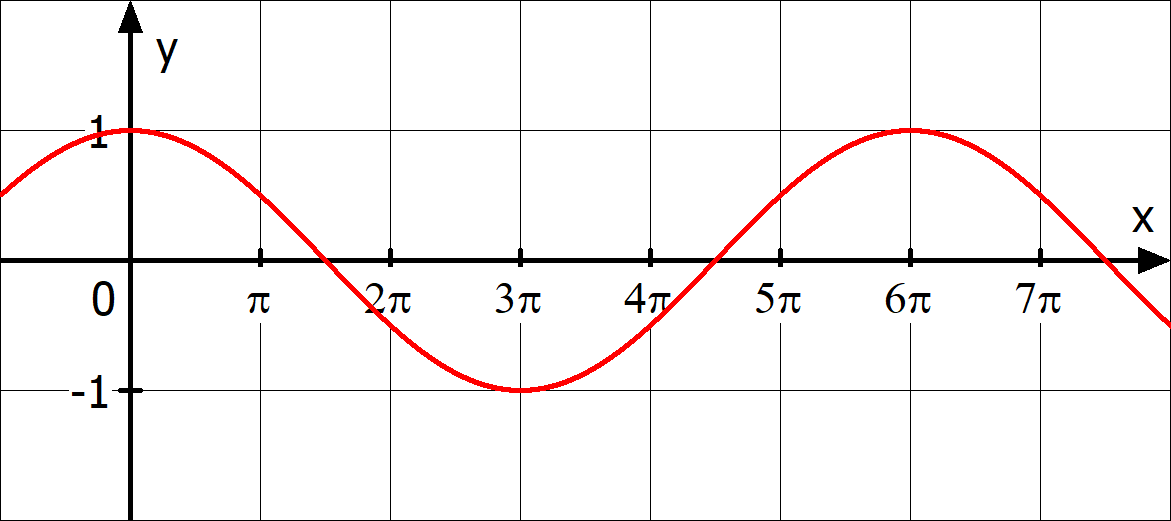
\includegraphics[height=5cm]{\trigonometrie/pics/AllgSinA1_4.png}\\
		\end{minipage}	 
		\item Amplitude \(a_{5}=1\), Periode \(p_{5}=4\pi\), Mittelwert \(d_{5}=-1\)\\
		\begin{minipage}{\textwidth}
			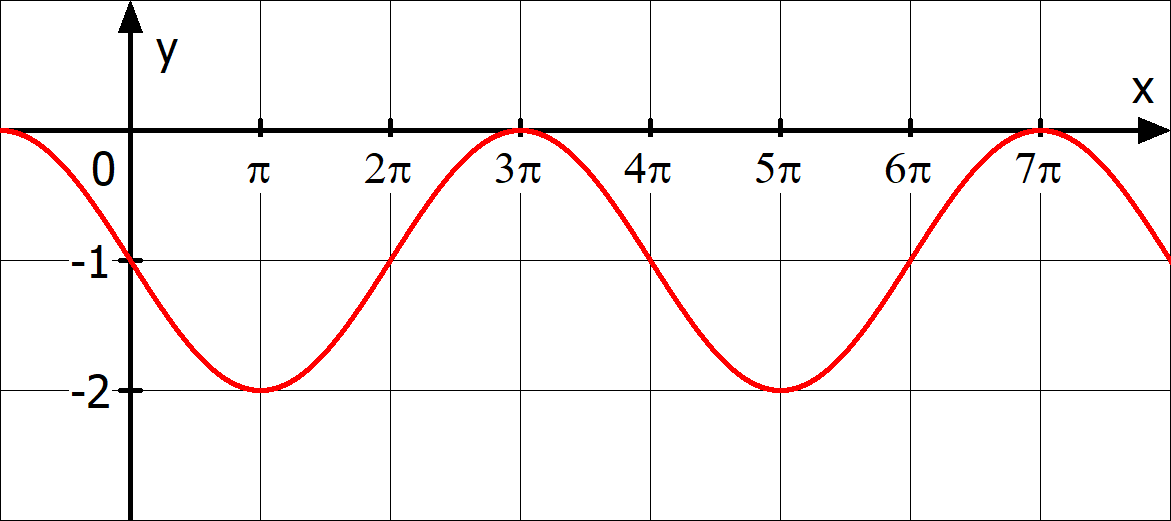
\includegraphics[height=5cm]{\trigonometrie/pics/AllgSinA1_5.png}\\
		\end{minipage}	 
		\item Amplitude \(a_{6}=3\), Periode \(p_{6}=3\pi\), Mittelwert \(d_{6}=3\)\\
		\begin{minipage}{\textwidth}
			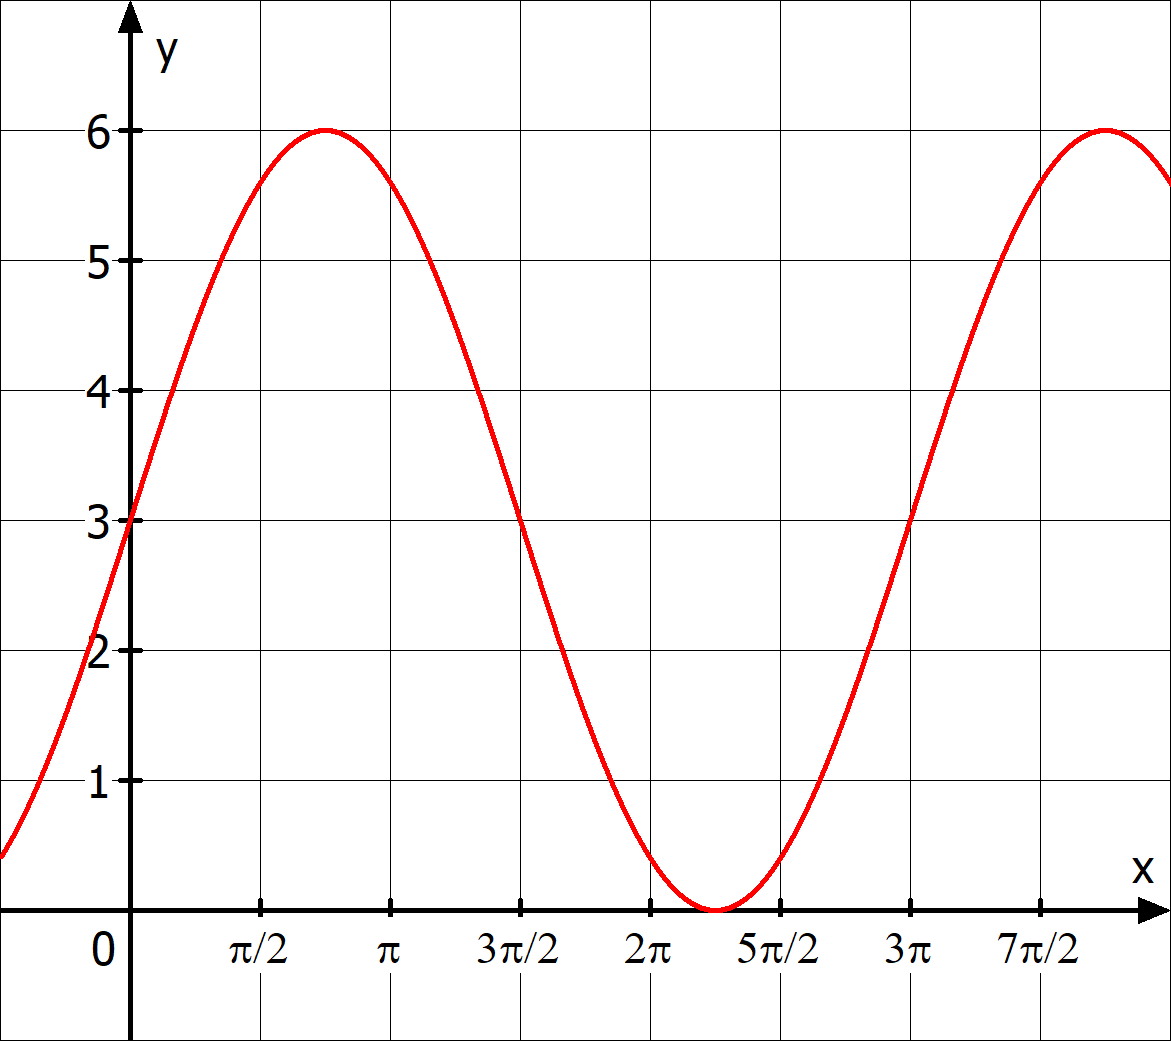
\includegraphics[height=5cm]{\trigonometrie/pics/AllgSinA1_6.png}\\
		\end{minipage}	 
		\item Amplitude \(a_{7}=4\), Periode \(p_{7}=\frac{8\pi}{3}\), Mittelwert \(d_{7}=2\)\\
		\begin{minipage}{\textwidth}
			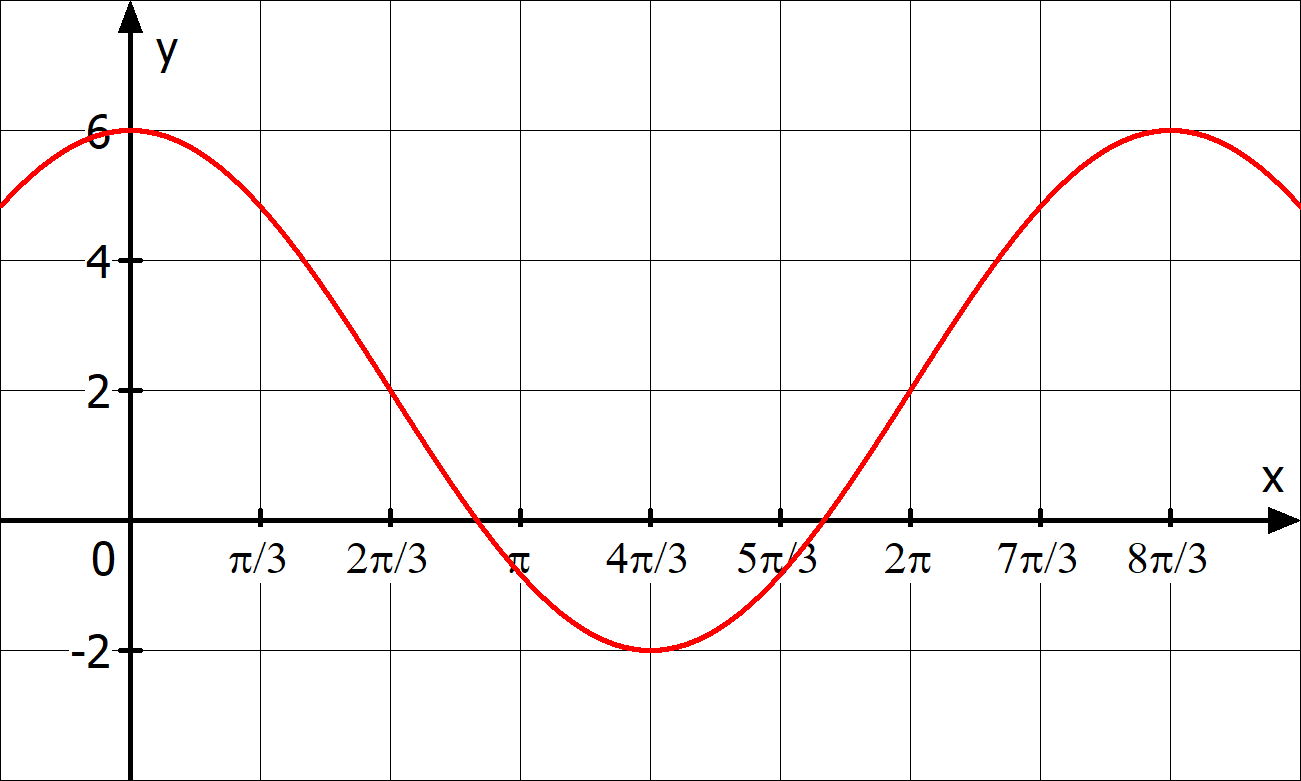
\includegraphics[height=5cm]{\trigonometrie/pics/AllgSinA1_7.png}\\
		\end{minipage}	 
		\item Amplitude \(a_{8}=2,5\), Periode \(p_{8}=2\), Mittelwert \(d_{8}=-1\)\\
		\begin{minipage}{\textwidth}
			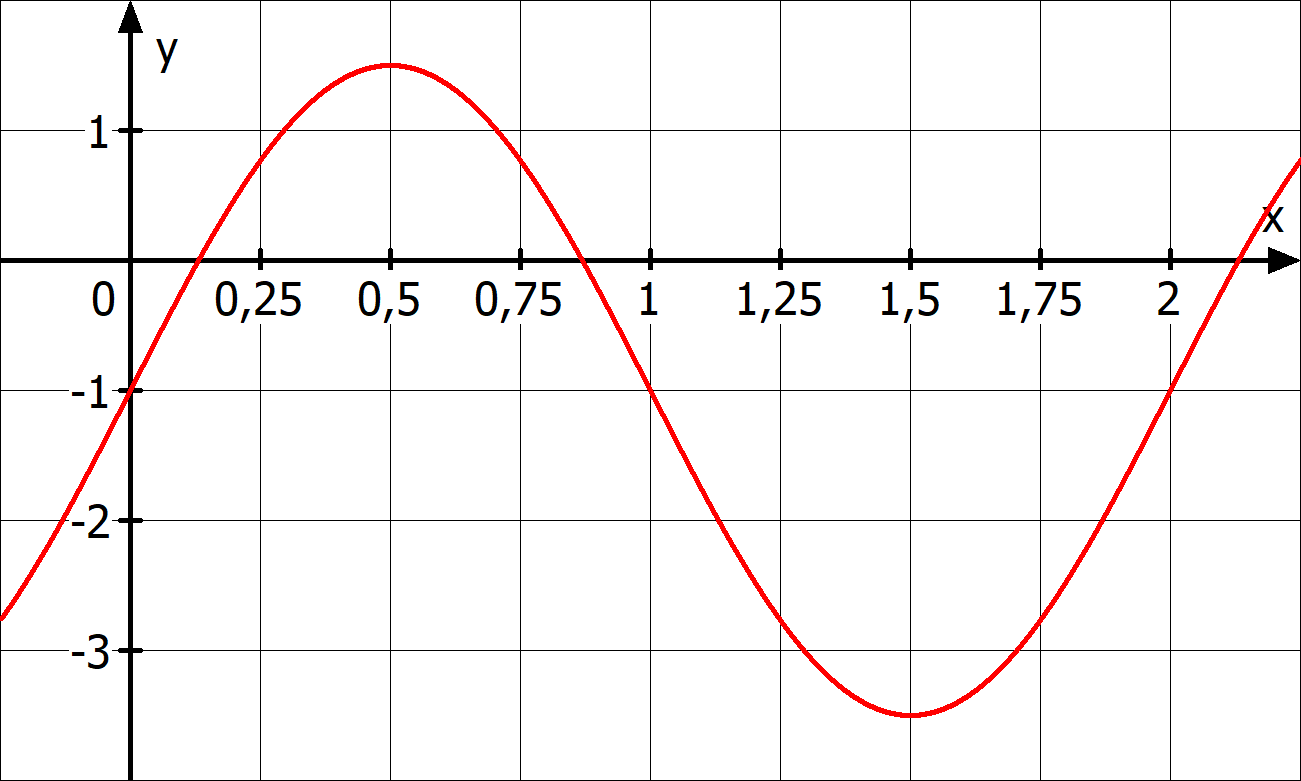
\includegraphics[height=5cm]{\trigonometrie/pics/AllgSinA1_8.png}\\
		\end{minipage}	\newpage
		\item Amplitude \(a_{9}=1\), Periode \(p_{9}=4\), Mittelwert \(d_{9}=2\)\\
		\begin{minipage}{\textwidth}
			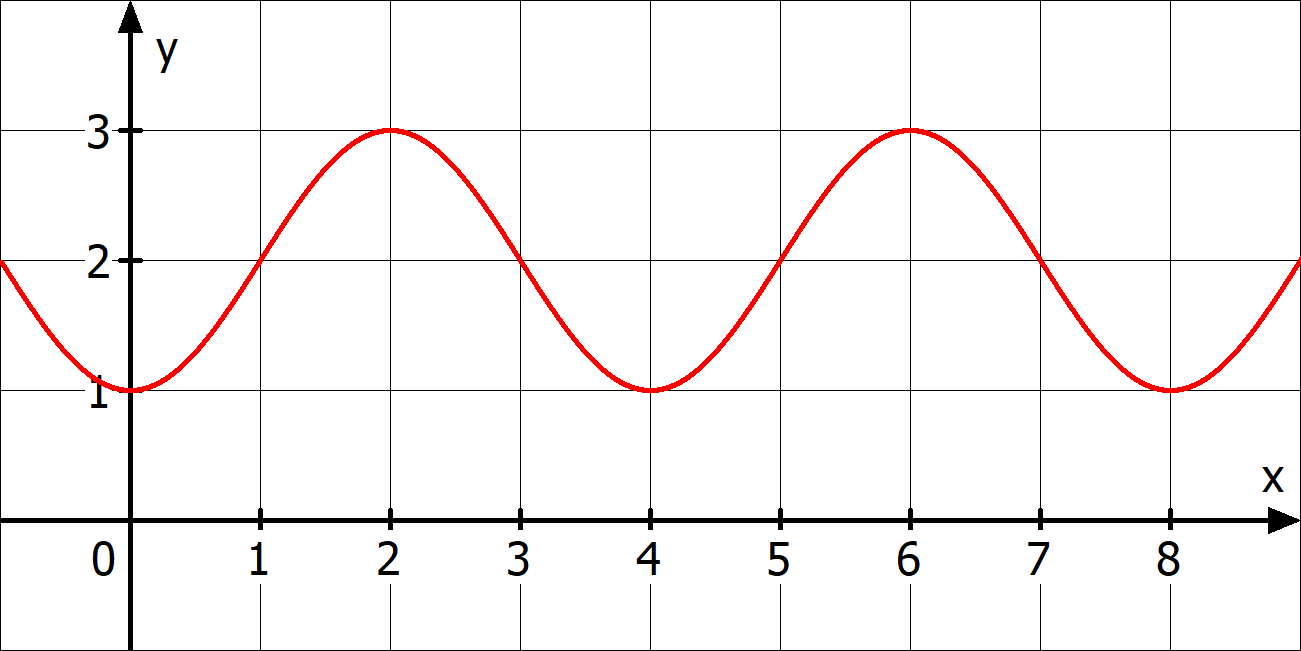
\includegraphics[height=5cm]{\trigonometrie/pics/AllgSinA1_9.png}\\
		\end{minipage}	 
		\item Amplitude \(a_{10}=4\), Periode \(p_{10}=1\), Mittelwert \(d_{10}=-1\)\\
		\begin{minipage}{\textwidth}
			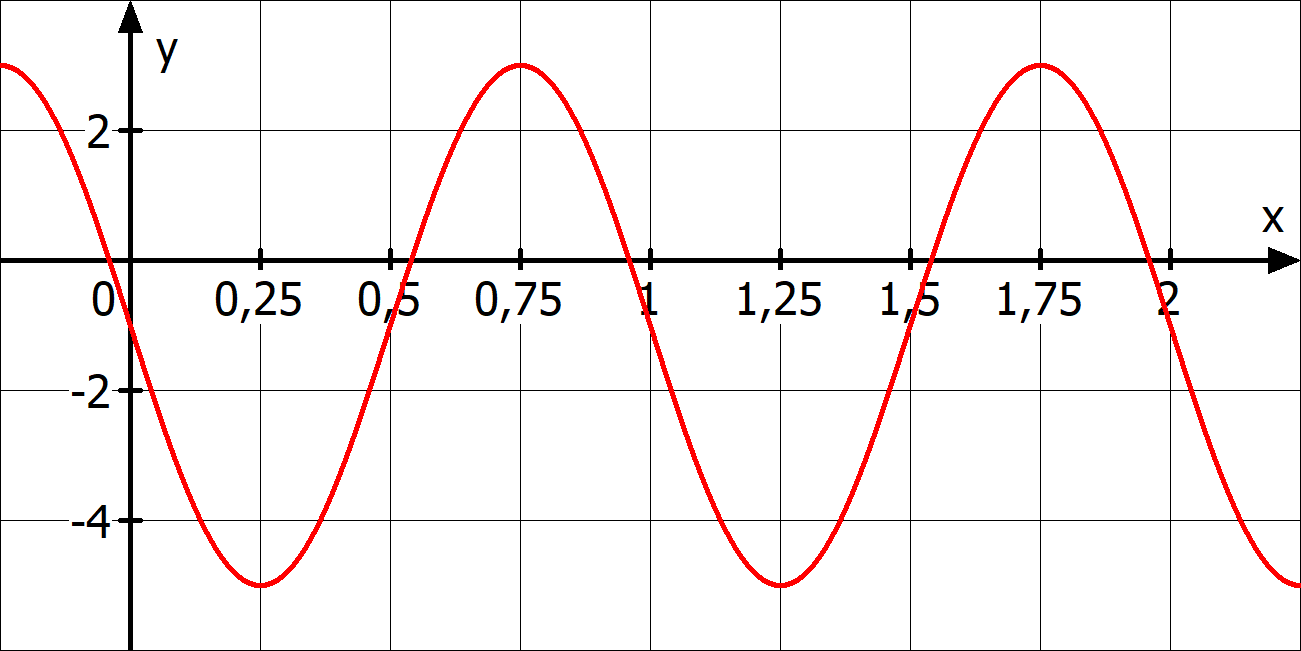
\includegraphics[height=5cm]{\trigonometrie/pics/AllgSinA1_10.png}\\
		\end{minipage}	 
		\item Amplitude \(a_{11}=2,5\), Periode \(p_{11}=\frac{1}{2}\), Mittelwert \(d_{11}=3,5\)\\
		\begin{minipage}{\textwidth}
			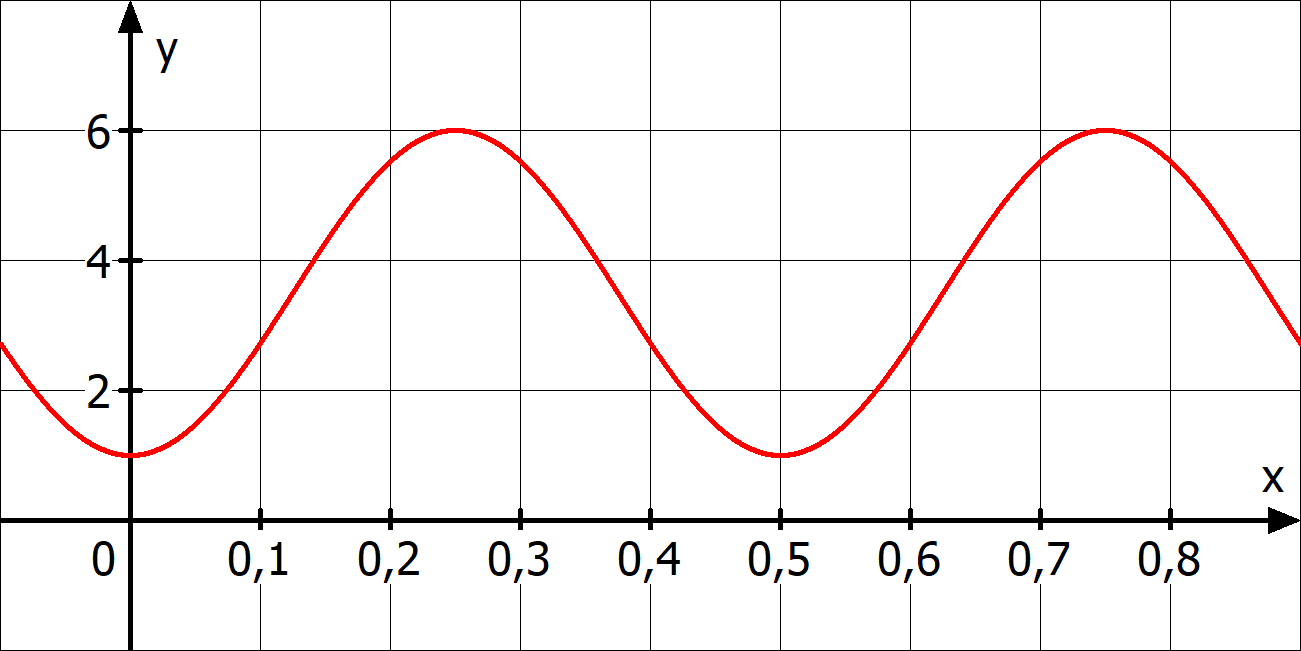
\includegraphics[height=5cm]{\trigonometrie/pics/AllgSinA1_11.png}\\
		\end{minipage}	 
		\item Amplitude \(a_{12}=3\), Periode \(p_{12}=\frac{4\pi}{3}\), Mittelwert \(d_{12}=2\)\\
		\begin{minipage}{\textwidth}
			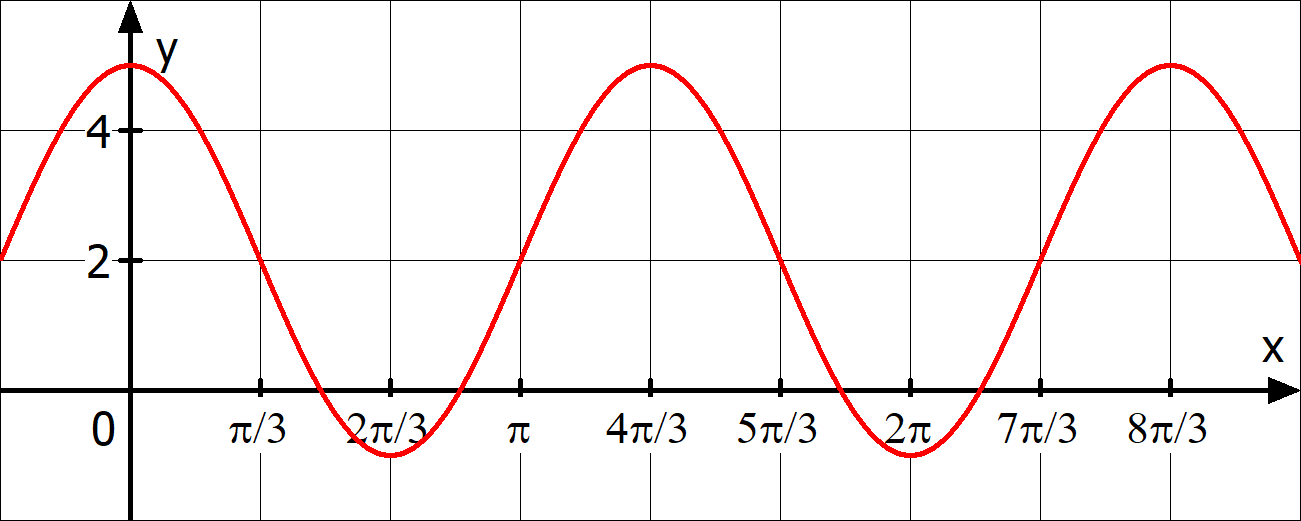
\includegraphics[height=5cm]{\trigonometrie/pics/AllgSinA1_12.png}\\
		\end{minipage}	 \newpage
		\item Amplitude \(a_{13}=0,5\), Periode \(p_{13}=4\), Mittelwert \(d_{13}=1,5\)\\
		\begin{minipage}{\textwidth}
			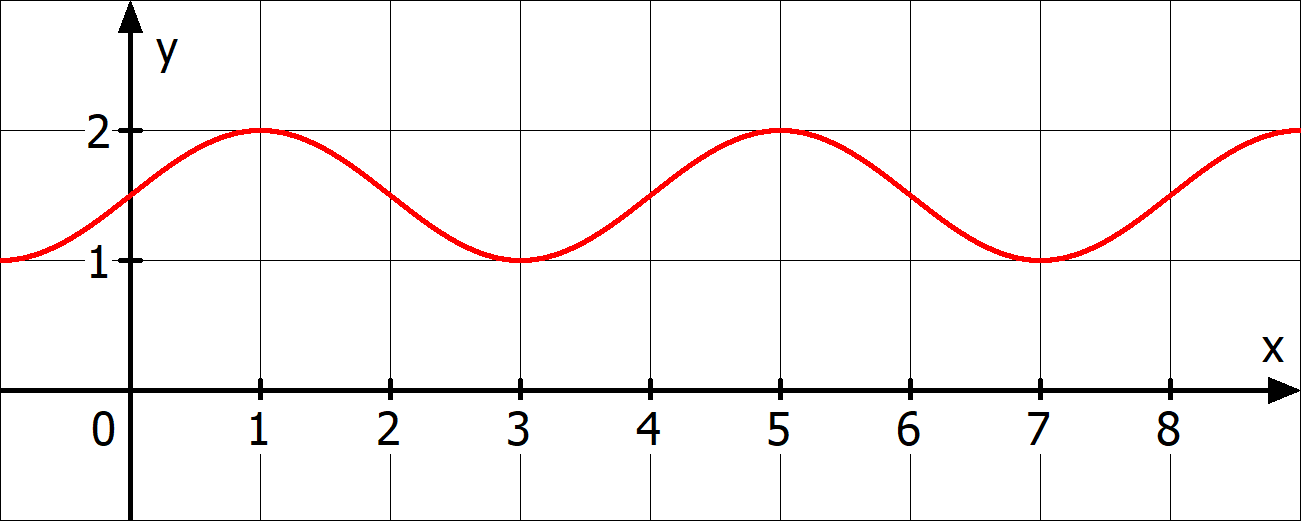
\includegraphics[height=5cm]{\trigonometrie/pics/AllgSinA1_13.png}\\
		\end{minipage}	 
		\item Amplitude \(a_{14}=5\), Periode \(p_{14}=0,5\), Mittelwert \(d_{14}=-3\)\\
		\begin{minipage}{\textwidth}
			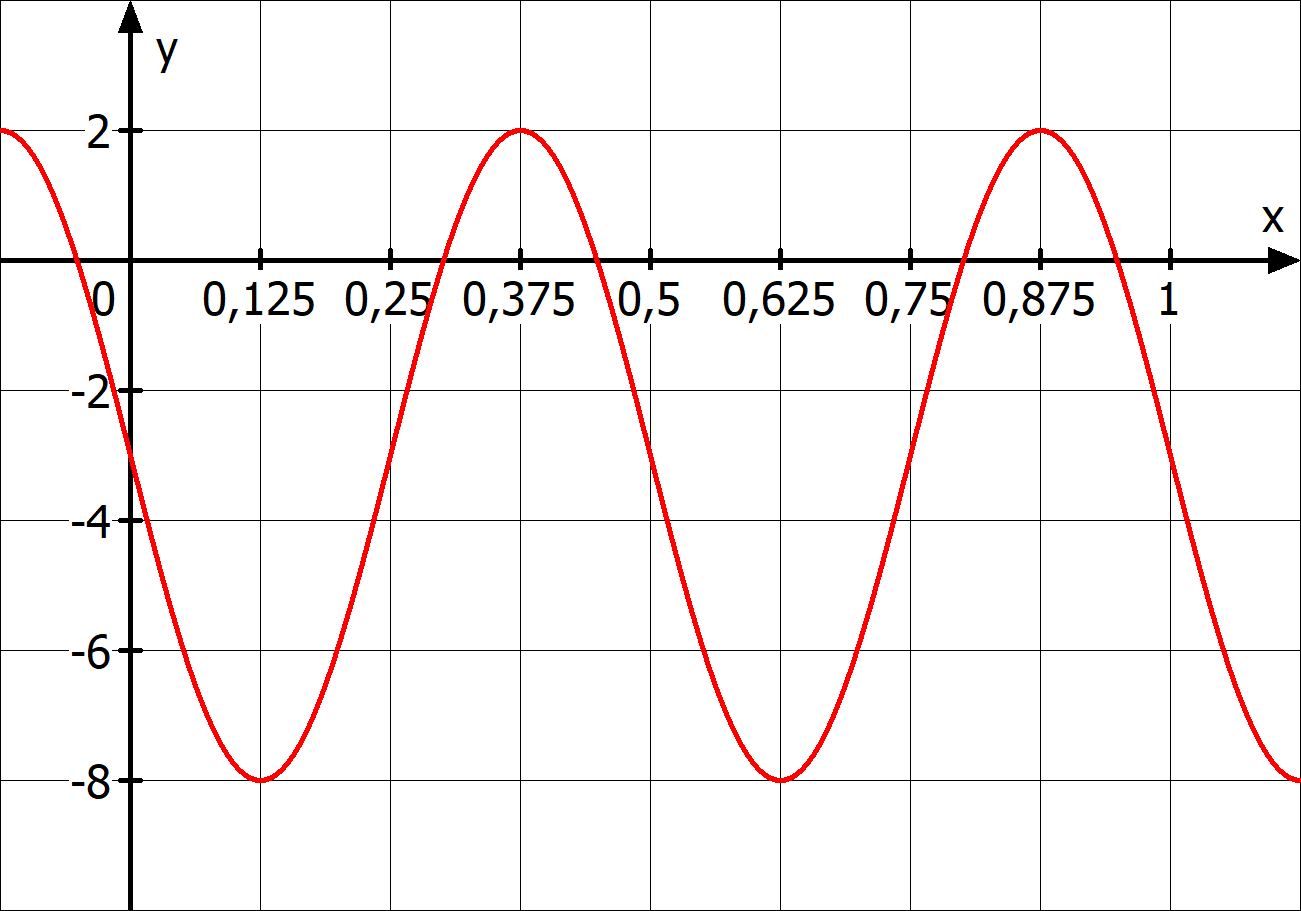
\includegraphics[height=5cm]{\trigonometrie/pics/AllgSinA1_14.png}\\
		\end{minipage}	 
		\item Amplitude \(a_{15}=3\), Periode \(p_{15}=2\pi\), Mittelwert \(d_{15}=2\)\\
		\begin{minipage}{\textwidth}
			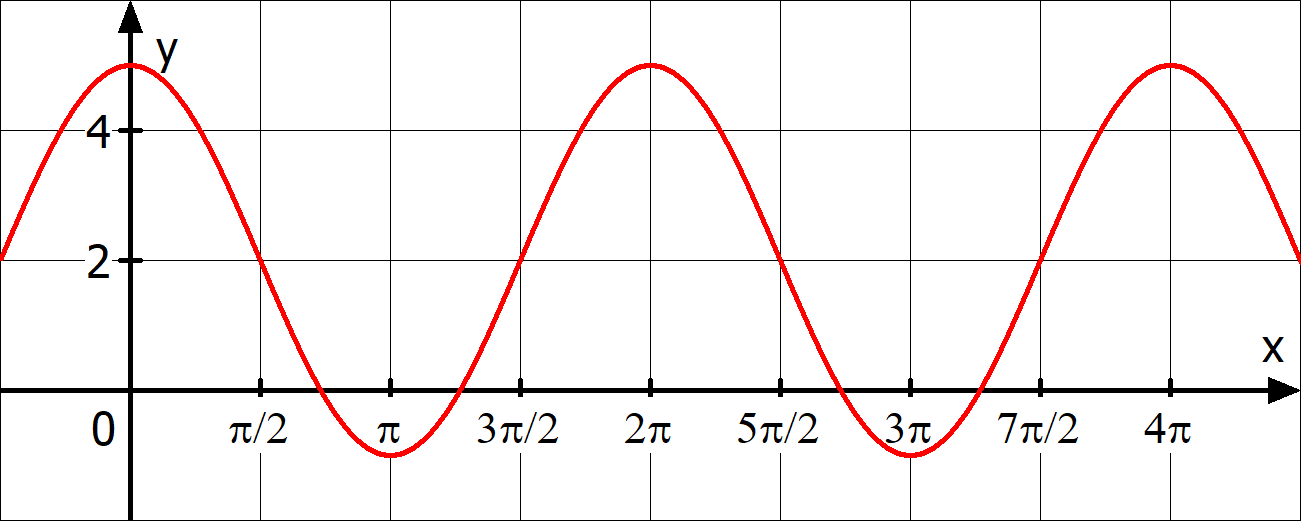
\includegraphics[height=5cm]{\trigonometrie/pics/AllgSinA1_15.png}\\
		\end{minipage}	 
		\item Amplitude \(a_{16}=2\), Periode \(p_{16}=\pi\), Mittelwert \(d_{16}=0\)\\
		\begin{minipage}{\textwidth}
			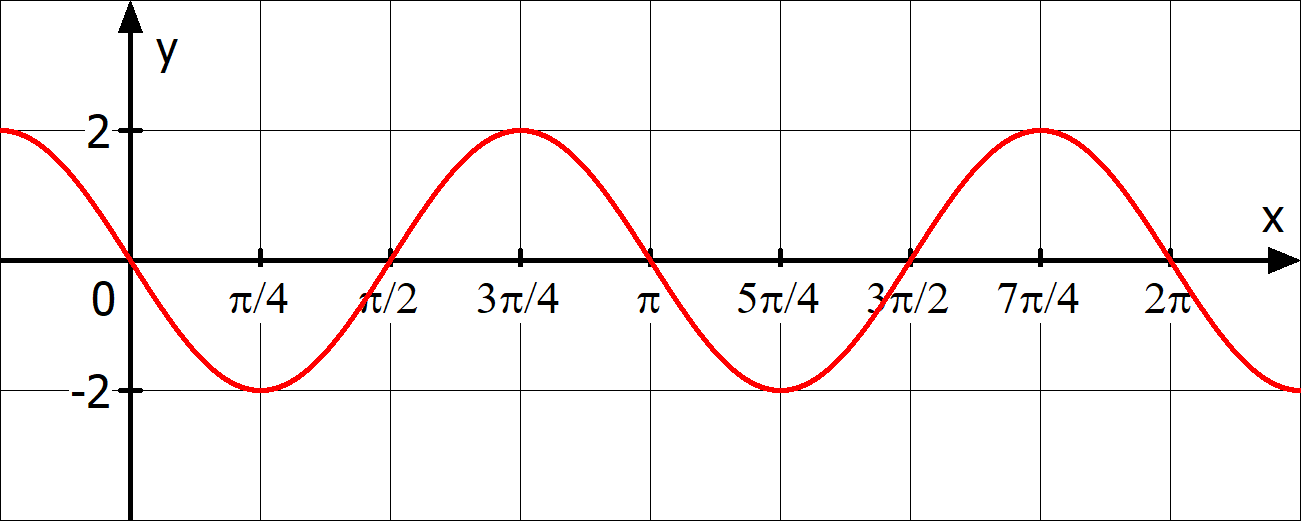
\includegraphics[height=5cm]{\trigonometrie/pics/AllgSinA1_16.png}\\
		\end{minipage}	 \newpage
		\item Amplitude \(a_{17}=2,5\), Periode \(p_{17}=\pi\), Mittelwert \(d_{17}=-3,5\)\\
		\begin{minipage}{\textwidth}
			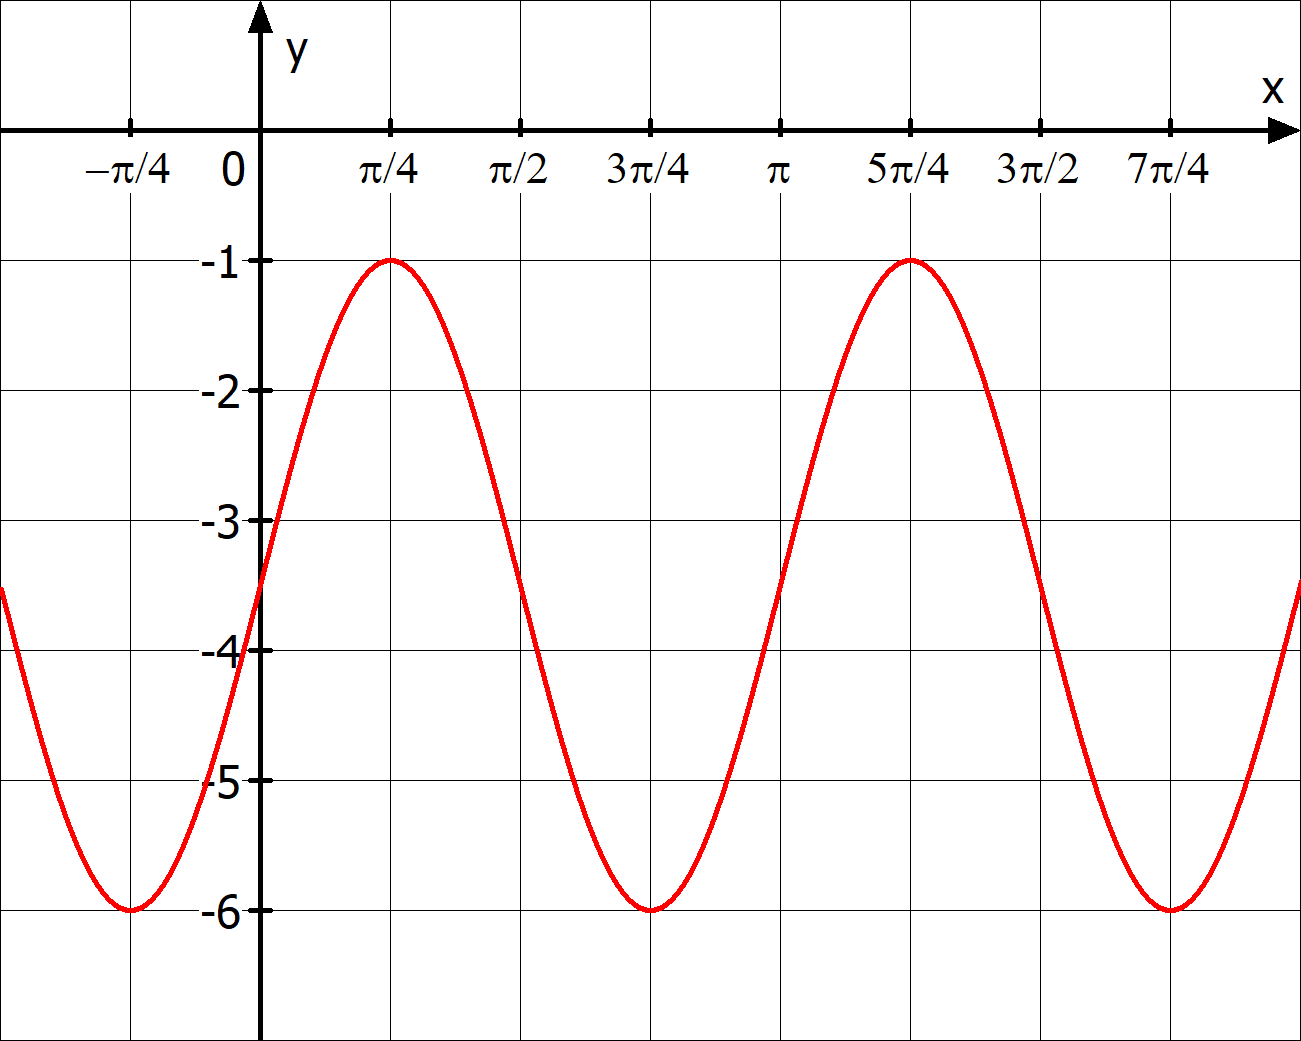
\includegraphics[height=5cm]{\trigonometrie/pics/AllgSinA1_17.png}\\
		\end{minipage}	 
		\item Amplitude \(a_{18}=3,5\), Periode \(p_{18}=3\), Mittelwert \(d_{18}=2\)\\
		\begin{minipage}{\textwidth}
			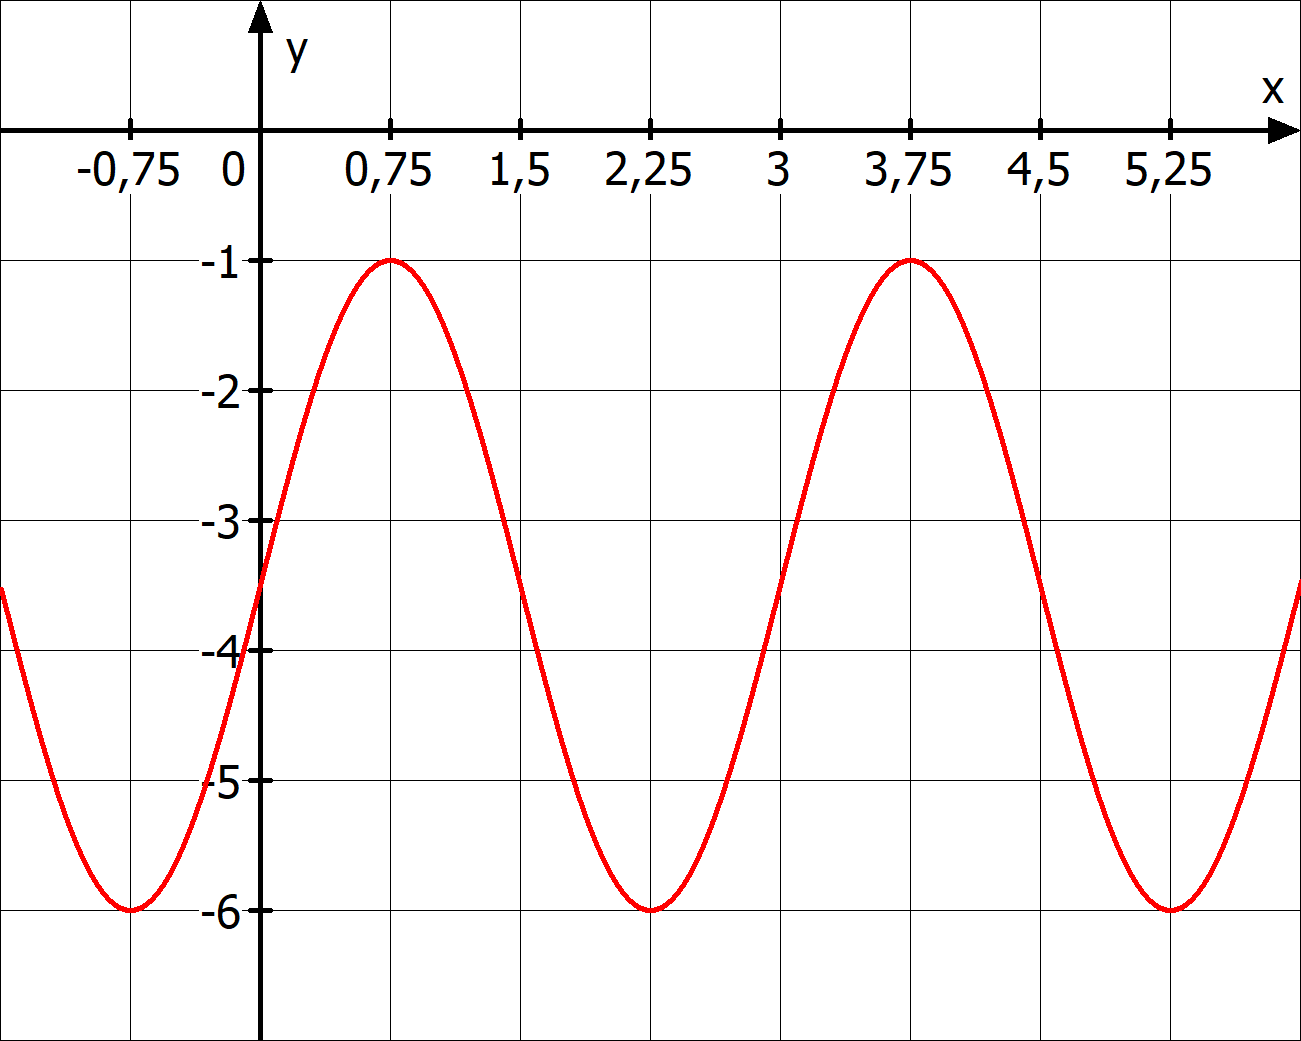
\includegraphics[height=5cm]{\trigonometrie/pics/AllgSinA1_18.png}\\
		\end{minipage}	 
		\item Amplitude \(a_{19}=5\), Periode \(p_{19}=2\pi\), Mittelwert \(d_{19}=-4\)\\
		\begin{minipage}{\textwidth}
			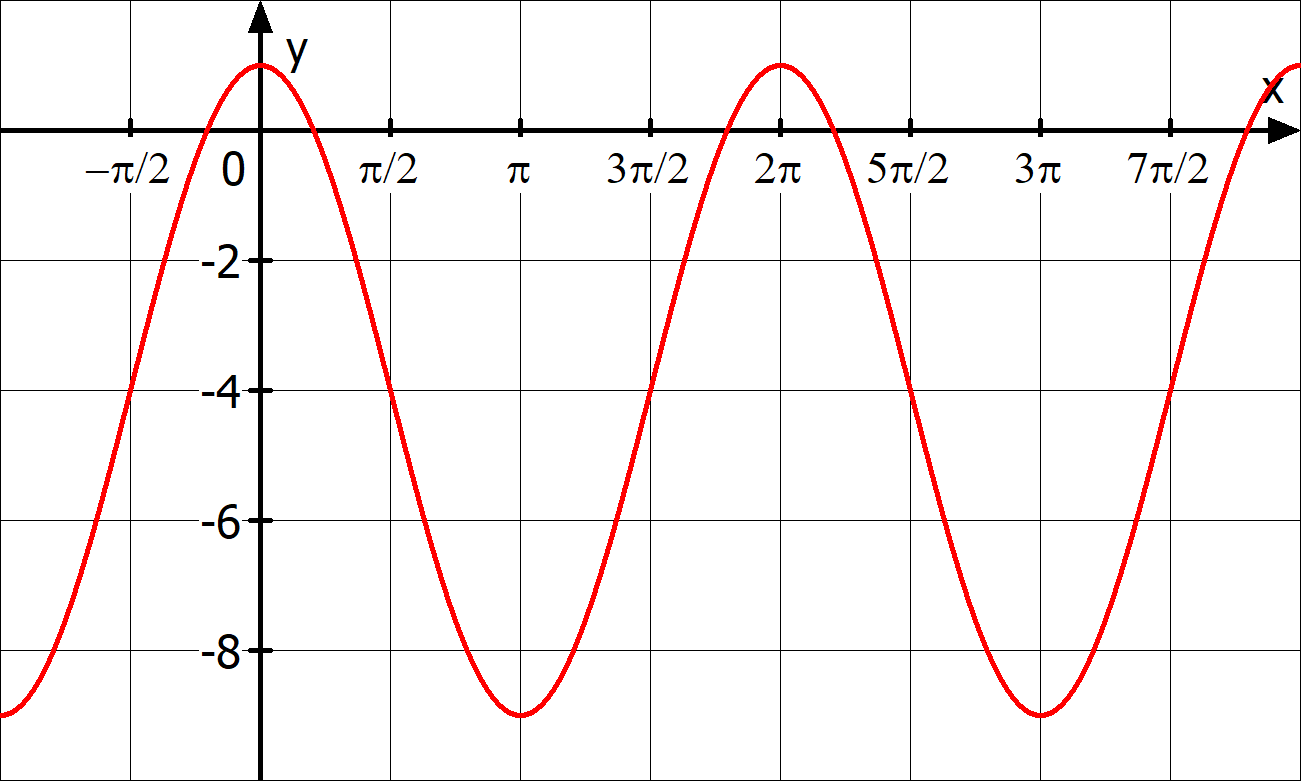
\includegraphics[height=5cm]{\trigonometrie/pics/AllgSinA1_19.png}\\
		\end{minipage}	 
		\item Amplitude \(a_{20}=6\), Periode \(p_{20}=1\), Mittelwert \(d_{20}=10\)\\
		\begin{minipage}{\textwidth}
			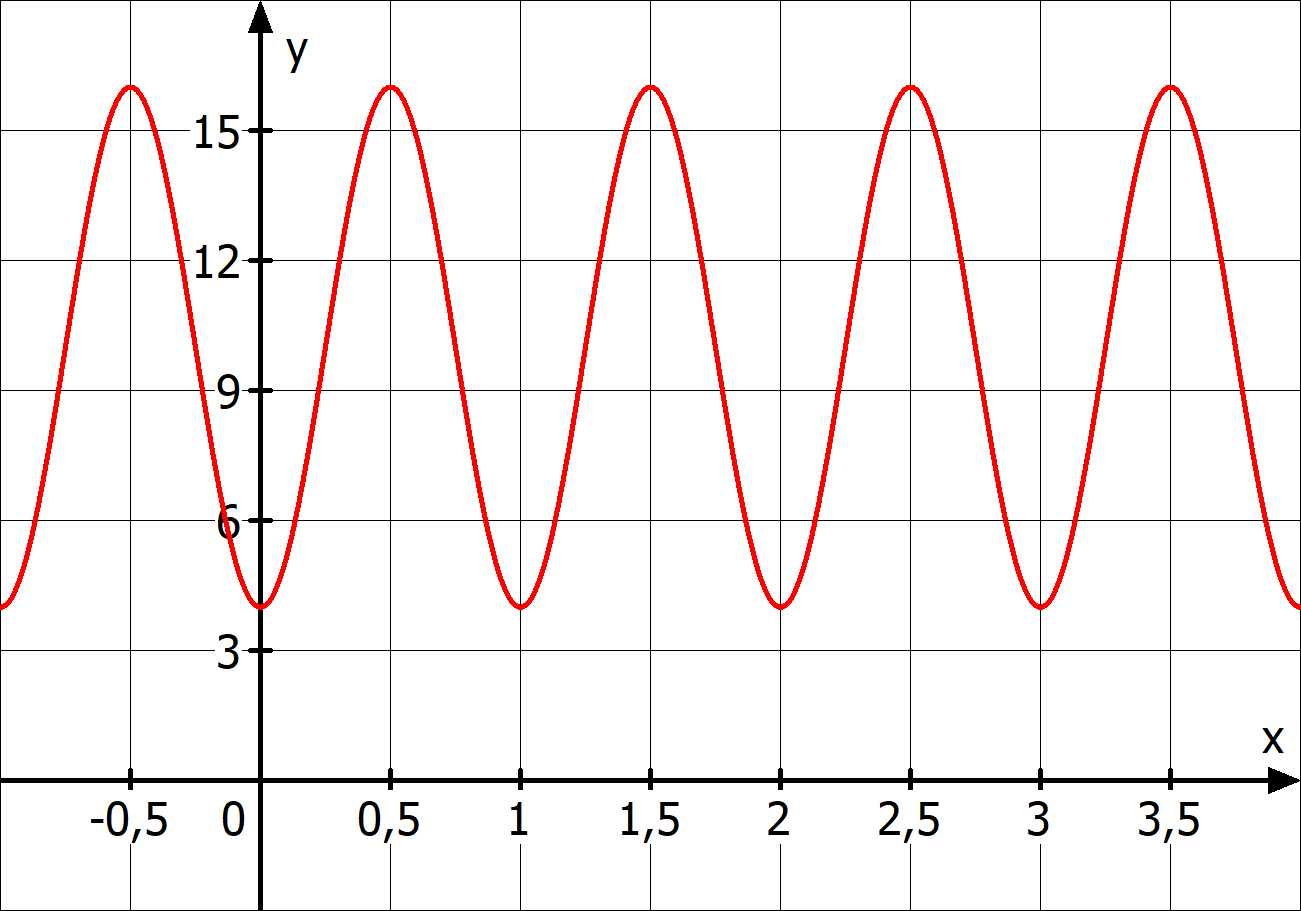
\includegraphics[height=5cm]{\trigonometrie/pics/AllgSinA1_20.png}\\
		\end{minipage}	 
	\end{enumerate}
\end{Answer}
\begin{Answer}[ref=allgSinCosA2]
	\begin{enumerate}[label=\alph*)]
		\item \(f_1(x)=2\sin\left(x\right)+1\)
		\item \(f_2(x)=-\sin\left(\frac{1}{2}x\right)-1\)
		\item \(f_3(x)=1,5\cos\left(\pi x\right)+0,5\)
		\item \(f_4(x)=-3\cos\left(2\pi x\right)+3\)
		\item \(f_5(x)=-\cos\left(4x\right)+2\)
		\item \(f_6(x)=-0,5\sin\left(\frac{3}{2}x\right)+1\)
		\item \(f_7(x)=\sin\left(\frac{3\pi}{2}x\right)-0,5\)
		\item \(f_8(x)=-3\sin\left(4\pi x\right)-1\)
		\item \(f_9(x)=-2,5\cos\left(2\pi x\right)-5\)
		\item \(f_{10}(x)=\sin\left(\frac{1}{4} x\right)-0,75\)
	\end{enumerate}
\end{Answer}